Chapter \ref{ch:naive} demonstrated that the modeling and
approximation techniques described in Chapter \ref{ch:algs} can be
used to model and predict numeric approximations of system
variability. The case study was only for four-dimensional data, and
the key weakness of the best predictor (Delaunay) is scaling with
dimension. This Chapter discusses a modeling approach that may achieve
better scaling with dimension, proposes a quasi-mesh construction, and
analyzes the performance of this proposed technique.


\section{Box Splines}
\label{sec_box_splines}

\begin{figure}
  \centering
  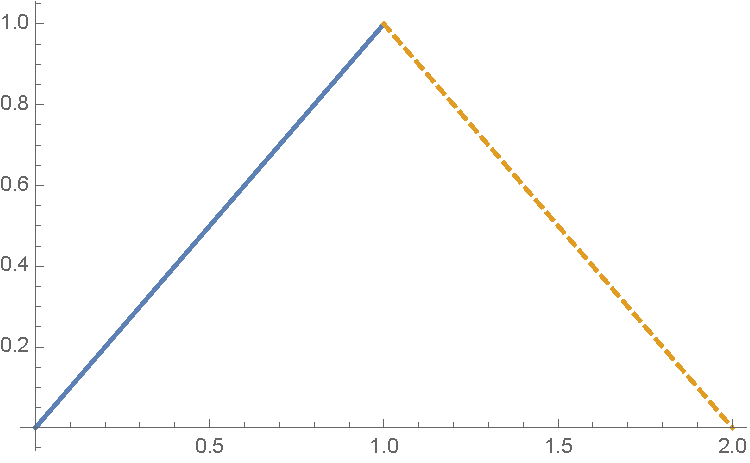
\includegraphics[width=0.45\textwidth]{Figures/ACM/1D-linear.pdf}
  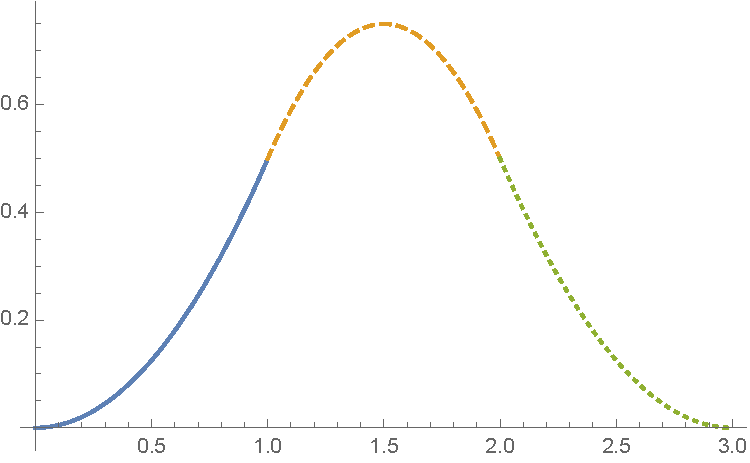
\includegraphics[width=0.45\textwidth]{Figures/ACM/1D-quadratic.pdf}
  \caption{1D linear (order 2) and quadratic (order 3) box splines with direction vector sets $\bigl( 1 \ 1 \bigr)$ and $\bigl( 1 \ 1 \ 1 \bigr)$ respectively. Notice that these direction vector sets form the B-Spline analogues, order 2 composed of two linear components and order 3 composed of 3 quadratic components (colored and styled in plot).}
  \label{fig_1D_boxes}
\end{figure}

\begin{figure}
  \centering
  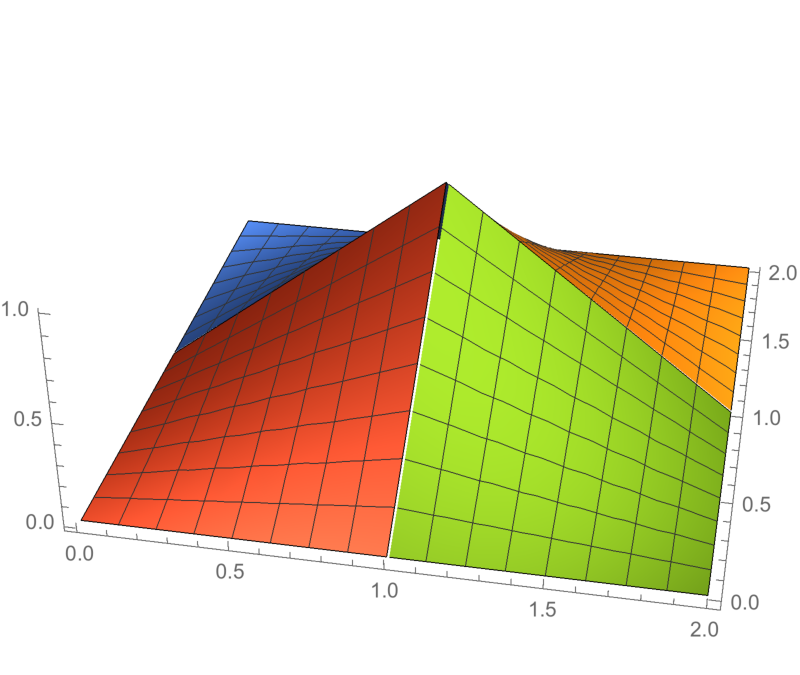
\includegraphics[width=0.45\textwidth]{Figures/ACM/2D-linear.pdf}
  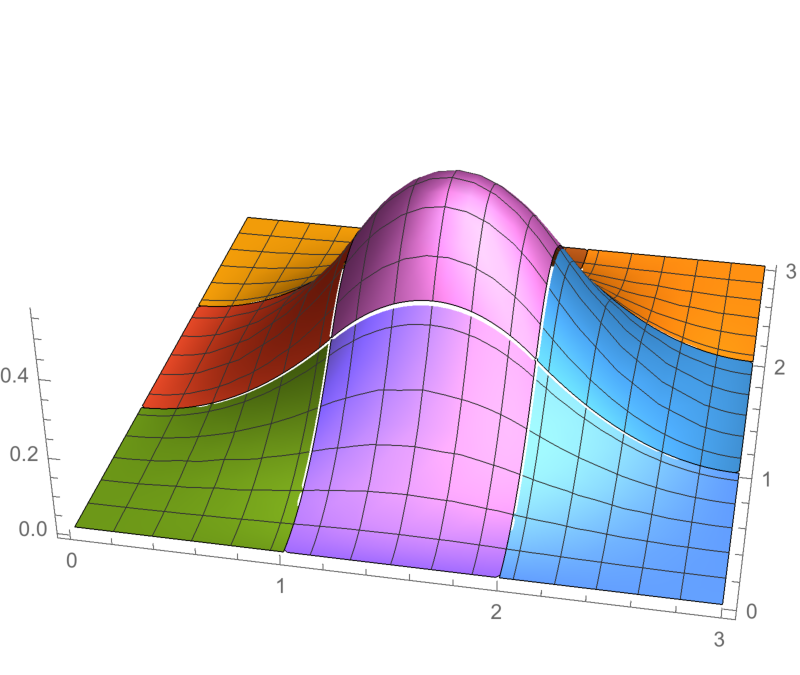
\includegraphics[width=0.45\textwidth]{Figures/ACM/2D-quadratic.pdf}
  \caption{2D linear (order 2) and quadratic (order 3) box splines with direction vector sets $\bigl( I \ I \bigr)$ and $\bigl( I \ I \ I \bigr)$ respectively, where $I$ is the identity matrix in two dimensions. Notice that these direction vector sets also produce boxes with $\text{order}^2$ subregions (colored in plot).}
  \label{fig_2D_boxes}
\end{figure}

A box spline in $\mathbb{R}^d$ is defined by its \textit{direction vector set} $A$, composed of $s$ $d$-vectors where $s \geq d$. Further, $A$ will be written as a $d \times s$ matrix. The first $m$ column vectors of $A$ are denoted by $A_m$, $m \leq s$. $A_d$ is required to be nonsingular. Consider the unit cube in $s$ dimensions $Q_s = [0,1)^s$. $A_s \bigl( Q_s \bigr)$ is now the image (in $d$ dimensions) of $Q_s$ under the linear map $A$. This image is the region of support for the box spline defined by $A_s$ in $d$ dimensions. The box spline function in $d$ dimensions for $A_d$ is defined as
\begin{equation}
B(x \mid A_d) = \begin{cases} 
(\det(A_d))^{-1}, & x \in A_d(Q_d), \\
0,                & \text{otherwise.}
\end{cases}
\label{eq_box_base}
\end{equation}
For $A_s$ when $s > d$ the box spline is computed as
\begin{equation}
B(x \mid A_s) = \int_0^1 B(x - t v_s \mid A_{s-1}) dt,
\label{eq_box_recursive}
\end{equation}
where $v_s$ is the $s$th direction vector of $A$.

The application of box splines presented in this chapter always utilizes the $d$-dimensional identity matrix as $A_d$. This simplifies the computation in Equation \ref{eq_box_base} to be the characteristic function for the unit cube. Composing $A$ strictly out of $k$ repetitions of the identity matrix forms the $k$th order B-spline with knots located at $0$, $1$, $\ldots$, $k-1$, $k$ along each axis (see Figure \ref{fig_1D_boxes}). Furthermore, while the number of subregions for the $k$th order $d$-dimensional box spline grows as $k^d$ (see Figure \ref{fig_2D_boxes}), the symmetry provided by direction vector sets composed of repeated identity matrices allows the computation of box splines to be simplified. The value of a box spline at any location is then the product of all axis-aligned 1-dimensional $k$th order box splines.

The box splines as presented are viable basis functions. Each box spline can be shifted and scaled without modifying the underlying computation (similar to wavelets), yet the underlying computation is simple and scales linearly with dimension. For a more thorough introduction and exploration of box splines in their more general form, readers are referred to \cite{de2013box}. 

\begin{figure}
  \centering
  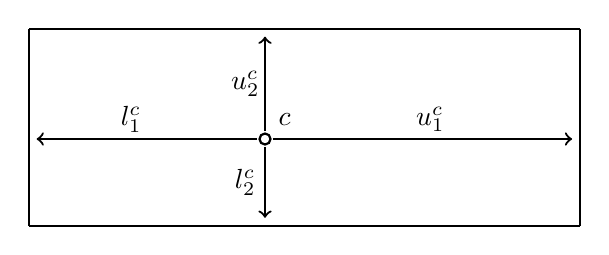
\begin{tikzpicture}[scale=1]
    \draw[thick] (3,1.1) circle (0.7mm);

    %% Draw arrows for each width
    \draw[thick,->] (3,1.2) -- (3,2.4);
    \draw[thick,->] (3,1.0) -- (3,0.1);
    \draw[thick,->] (3.1,1.1) -- (6.9,1.1);
    \draw[thick,->] (2.9,1.1) -- (0.1,1.1);

    %% Draw boundary of box
    \draw[thick,-] (0,0) -- (7,0);
    \draw[thick,-] (7,0) -- (7,2.5);
    \draw[thick,-] (7,2.5) -- (0,2.5);
    \draw[thick,-] (0,2.5) -- (0,0);

    %% Add text to the picture
    \node at (3.25,1.35) {$c$};
    \node at (1.3,1.35) {$l^c_1$};
    \node at (5.1,1.35) {$u^c_1$};
    \node at (2.75,0.55) {$l^c_2$};
    \node at (2.75,1.8) {$u^c_2$};
  \end{tikzpicture}
  \caption{An example box in two dimensions with anchor $c$, upper widths $u^c_1$, $u^c_2$, and lower widths $l^c_1$, $l^c_2$. Notice that $c$ is not required to be equidistant from opposing sides of the box, that is $u^c_i \not= l^c_i$ is allowed.}
  \label{fig_example_box}
\end{figure}

Throughout this section, the notation will be reused from Chapter \ref{ch:algs}. $X \subset \mathbb{R}^d$ is a finite set of points with known response values $f(x)$ for all $x \in X$. Also let $L,U \in \mathbb{R}^d$ define a bounding box for $X$ such that $L < x < U$ for all $x \in X$.

Define a box $b^c = (c,l^c,u^c)$ in $d$ dimensions with anchor $c \in \mathbb{R}^d$, lower width vector $l^c \in \mathbb{R}^d_+$, and upper width vector $u^c \in \mathbb{R}^d_+$ (where $u^c_i$ refers to the $i$th component of $u^c$). A visual example of a box in two dimensions can be seen in Figure \ref{fig_example_box}. Now, define a componentwise rescaling function $g: \mathbb{R}^d \rightarrow \mathbb{R}^d$ at point $x \in \mathbb{R}^d$ to be
\begin{equation}
  \bigl(g^c(x)\bigr)_r = {k \over 2} \left( 1 - {(x_r - c_r)_- \over l^c_r} + {(x_r - c_r)_+ \over u^c_r} \right),
\end{equation}
where $y_+=\max\{y,0\}$, $y_-=(-y)_+$, $k$ is the order of the box spline as described in Section \ref{sec_box_splines}. Finally, each box spline in a box mesh can be evaluated as $B^c(x) = B(g^c(x) \mid A)$ presuming the order of approximation implies $A$. Both box meshes described in the following sections use box spline basis functions of this form.

A notable property of boxes defined with the linear rescaling function $g^c$, is that $C^0$ and $C^1$ continuity of the underlying box spline are maintained. $C^0$ continuity is maintained through scaling. $C^1$ continuity is maintained for all box splines with $C^1$ continuity (order $\geq 3$) because the scaling discontinuity is located at $c$, where all box splines (of the presented form) have first derivative zero. All continuity beyond the first derivative is lost through the rescaling function $g^c$.

\section{Max Box Mesh}

The first of the three meshes produces a set of boxes around chosen control points and each box has maximal distance between the control point and the nearest side of the box. This centrality property is one mechanism for creating the largest reasonable regions of support for the underlying basis functions. The individual boxes are constructed via the following procedure given a set of control points $C \subseteq X$, $c^{(i)} \in C$,
\begin{enumerate}
  \item Initialize a box $b^{c^{(1)}} = \bigl(c^{(1)}, (c^{(1)} - L), (U - c^{(1)})\bigr)$. \label{step_init}
  \item Identify $c^{(i)}$ over $\bigl\{ j \bigm| j \ne 1$, $B^{c^{(1)}}\bigl( c^{(j)} \bigr) \ne 0 \bigr\}$ that minimizes $\bigl\|c^{(j)}-c^{(1)}\bigr\|_\infty$.  \label{step_closest}
  \item Change the the box $b^{c^{(1)}}$ along the first dimension $r$ such that $\bigl|\bigl|c^{(1)} - c^{(i)}\bigr|\bigr|_\infty = \bigl\vert c^{(1)} - c^{(i)}\bigr\vert_r $, to exclude $c^{(i)}$ from the support of $B^{c^{(1)}}$. \label{step_shrink}
  \item Repeat steps \ref{step_closest} and \ref{step_shrink} until no point in $C$ is in the support of $B^{c^{(1)}}$ (at most $2d$ times, once for each boundary of a box).
\end{enumerate}

The same process is used to construct boxes around all control points in $C$. In order to improve the generality of the approximation, a set of control points is initially chosen to be well-spaced using a statistical method from \citet{amos2014algorithm}:

\begin{enumerate}
\item Generate a sequence of all pairs of points sorted by ascending pairwise Euclidean distance between points $\bigl(x^{(i_1)},x^{(j_1)}\bigr)$, $\bigl(x^{(i_2)},x^{(j_2)}\bigr)$, $\ldots$ , so that $\bigl\|x^{(i_k)}-x^{(j_k)}\bigr\|_2 \leq \bigl\|x^{(i_{k+1})}-x^{(j_{k+1})}\bigr\|_2$.
\item Sequentially remove points from candidacy until only $|C|$ remain by randomly selecting a single point from each pair $\bigl(x^{(i_m)}, x^{(j_m)}\bigr)$ for $m = 1,\ldots$ if both $x^{(i_m)}$ and $x^{(j_m)}$ are still candidates for removal.
\end{enumerate}

Once the boxes for a max box mesh have been constructed, the parameters can be identified via a least squares fit. The max box mesh (denoted $MBM$) is used to generate a $|X| \times |C|$ matrix $M$ of box spline basis function evaluations at all points in $X$. The solution to the least squares problem $\min_P \bigl\| M \ P - f(X) \bigr\|_2$ is the parameterization of $MBM$. When $C = X$, $M$ is the $|X| \times |X|$ identity matrix, making the max box mesh approximation $\hat f$ an interpolant.

While setting the number of boxes equal to the number of points causes the max box mesh to be an interpolant, the generality of the max box mesh approximation can often be improved by bootstrapping the selection of control points. Given a user-selected batch size $s \leq |X|$, start with $s$ well-spaced control points. Next, measure the approximation error at $x \notin C$ and if the error is too large (determined by user), pick $s$ points at which the magnitude of approximation error is largest, add those points to $C$, and recompute the max box mesh. The user is left to decide the batch size $s$ and the error tolerance based on validation performance and computability. This work uses a batch size of one.

\begin{definition}
The hyperplane $x_r = c_r + u^c_r$ is the upper boundary of box $b^c$ along dimension $r$, and similarly $x_r = c_r - l^c_r$ is the lower boundary of box $b^c$. When the anchor point $y$, for some box $b^y$, lies in the hyperplane (and facet of box $b^c$) defining either boundary along dimension $r$ of $b^c$ it is said that $b^y$ \textit{bounds} $b^c$ in dimension $r$ and is denoted $\bigl( b^c \bigm\vert_r b^y \bigr)$.
\end{definition}

Throughout all experiments and all repeated trials conducted for this study, all tested interpolation points were covered by at least one box in the $MBM$. However, it is possible for the $MBM$ to not form a covering of $[L,U]$ when there are cyclic boundaries. Consider the following example in three dimensions:
\begin{align*}
  C         &= \bigl\{(0,0,0), (1,0,2/3), (1,1,4/3)\bigr\}, \\
  b^{c^{(1)}} &= \bigl( (0,0,0),  \ (*,*,*),  \ (1,*,4/3) \bigr), \\
  b^{c^{(2)}} &= \bigl( (1,0,2/3),\ (1,*,*),  \ (*,1,*)   \bigr), \\
  b^{c^{(3)}} &= \bigl( (1,1,4/3),\ (*,1,4/3),\ (*,*,*)   \bigr).
\end{align*}
Asterisks are used to represent boxes that are not bounded by other boxes along some dimensions. The point $(2,2,-3)$ is not in any of the max boxes defined above. In this case, there is a cycle in box boundaries that looks like $\bigl( b^{c^{(1)}} \bigm\vert_1 b^{c^{(2)}} \bigm\vert_2 b^{c^{(3)}} \bigm\vert_3 b^{c^{(1)}} \bigr)$. This example demonstrates that it is geometrically possible for the max box mesh to fail to cover a space, however experiments demonstrate that it is empirically unlikely.

The max box mesh remains a viable strategy for computed approximations. Given a maximum of $c$ control points in $d$ dimensions with $n$ points, the computational complexities are: $\mathcal{O}(c^2 d)$ for computing boxes, $\mathcal{O}(c d^2 + d^3)$ for a least squares fit, and $\mathcal{O}(n / s)$ for bootstrapping (which is multiplicative over the fitting complexities). Evaluating the max box mesh requires $\mathcal{O}(c d)$ computations.

\section{Iterative Box Mesh}

The iterative box mesh ($IBM$) comprises box-shaped regions that each contain exactly one control point in their interior just as in the $MBM$. However, the mesh is a covering for $[L,U]$ by construction and places boxes in a way that reduces apparent error. The boxes are constructed via the following procedure given a finite set of points $X \subset \mathbb{R}^d$, where $C \subseteq X$ is the (initially empty) set of control points.
\begin{enumerate}
\item Add the box that covers $[L,U]$ anchored at the most central point $x^{(k)} \in X$, add $x^{(k)}$ to $C$, and least squares fit the $IBM$ model to all $x \in X$.
\item Add a new box $[L,U]$ anchored at $x^{(i)} \notin C$ such that $\bigl| IBM(x^{(i)}) - f(x^{(i)}) \bigr| = \max_{x \in X \backslash C} \bigl| IBM(x) - f(x) \bigr|$, reshaping all boxes $b^{x^{(j)}}$ that contain $x^{(i)}$ by bounding the first dimension $r$ such that $\bigl| x^{(j)}_r - x^{(i)}_r \bigr| = \bigl\| x^{(j)} - x^{(i)} \bigr\|_\infty$ (also reshaping the box $b^{x^{(i)}}$ symmetrically), add $x^{(i)}$ to $C$, and then least squares fit the $IBM$ model to all $x \in X$. \label{step_add_box}
\item Repeat Step \ref{step_add_box} until model approximation error is below tolerance $t$.
\end{enumerate}

Just as for the $MBM$, the parameters can be identified via a least squares fit. The iterative box mesh is used to generate a $|X| \times |C|$ matrix $M$ of box spline function evaluations at all points in $X$. Now the box spline coefficients are the solution to the least squares problem $\min_P \bigl|\bigl| M\ P - f(X) \bigr|\bigr|_2$. Also as for the $MBM$, $C = X$ causes $M$ to equal the $|X| \times |X|$ identity, making the iterative box mesh approximation $\hat f$ an interpolant.

As opposed to the max box mesh, the bootstrapping procedure is built into the iterative box mesh. The user is left to decide the most appropriate error tolerance, however a decision mechanism and analysis is presented in Section \ref{sec_performance_analysis}. As mentioned earlier, the iterative box mesh is a covering for $[L,U]$ by construction and this can be proved by an inductive argument.

An $IBM$ least squares fit $\hat f(z) = \sum_{j}P_j B^{c^{(i_j)}}(z)$ can generate approximations at new points $z \in Z \subset \mathbb{R}^d$ by evaluating $\hat f(z)$. The computational complexity for generating the mesh is $\mathcal{O}(c^2 n d)$ where $c$ is the number of control points determined by the minimum error threshold and $n = |X|$. The computational complexity of evaluating the mesh at a single point is $\mathcal{O}(c d)$.

\section{Voronoi Mesh}

The final of the three meshes utilizes 2-norm distances to define boundaries rather than max norm distances. It also does not rely on box splines as the underlying basis function. A well-studied technique for classification and approximation is the nearest neighbor algorithm \cite{cover1967nearest}. Nearest neighbor inherently utilizes the convex region $v^{x^{(i)}}$ (Voronoi cell \cite{dirichlet1850reduction}) consisting of all points closer to $x^{(i)}$ than any other point $x^{(j)}$. The Voronoi mesh smooths the nearest neighbor approximation by utilizing the Voronoi cells to define support via a generic basis function $V: \mathbb{R}^d \rightarrow \mathbb{R}_+$ given by

$$ V^{x^{(i)}}(y) = \left(1 - \frac{\bigl\|y - x^{(i)}\bigr\|_2}{2 \ d(y \mid x^{(i)})} \right)_+, $$
where $x^{(i)}$ is the center of the Voronoi cell, $y \in \mathbb{R}^d$ is an interpolation point, and $d(y \mid x^{(i)})$ is the distance between $x^{(i)}$ and the boundary of the Voronoi cell $v^{x^{(i)}}$ in the direction $y - x^{(i)}$. $V^{x^{(i)}}\bigl(x^{(j)}\bigr) = \delta_{ij}$ and $V^{x^{(i)}}$ has local support. While $V^{x^{(i)}}(x^{(i)}) = 1$, the $2$ in the denominator causes all basis functions to go linearly to $0$ at the boundary of the twice-expanded Voronoi cell. Note that this basis function is $C^0$ because the boundaries of the Voronoi cell are $C^0$. In the case that there is no boundary along the vector $w$, the basis function value is always $1$.

While the cost of computing the exact Voronoi cells for any given set of points grows exponentially \cite{dutour2009complexity}, the calculation of $d$ is linear with respect to the number of control points and dimensions. Given any center $x^{(i)} \in \mathbb{R}^d$, set of control points $C \subseteq X$, and interpolation point $y \in \mathbb{R}^d$, $d\bigl(y \mid x^{(i)}\bigr)$ is the solution to
\begin{equation}
  \max_{c \in C\backslash\{x^{(i)}\}} \frac{\bigl\|y - x^{(i)}\bigr\|_2}{2} \ \frac{y \cdot \bigl(c - x^{(i)}\bigr) - x^{(i)} \cdot \bigl(c - x^{(i)}\bigr)}{c \cdot \bigl(c - x^{(i)}\bigr) - x^{(i)} \cdot \bigl(c - x^{(i)}\bigr)}.
\end{equation}

The parameters of the $VM$ can now be computed exactly as for the $MBM$ and $IBM$. The Voronoi mesh is used to generate a $|X| \times |C|$ matrix $M$ of basis function evaluations at all points in $X$. Now the $VM$ coefficients are the solution to the least squares problem $\min_P \bigl\| M \ P - f(X) \bigr\|_2$. When $X = C$, $M$ is the identity making the mesh an interpolant. Bootstrapping can be performed with an identical procedure to that for the $IBM$.
\begin{enumerate}
\item Pick the most central point $x^{(k)} \in X$ to be the first control point in $C$ and fit the $VM$ model to all $x \in X$.
\item Identify a control point $x^{(i)} \notin C$ such that $\bigl| VM(x^{(i)}) - f(x^{(i)}) \bigr| = \max_{x \in X \backslash C} \bigl| VM(x) - f(x) \bigr|$, add $x^{(i)}$ to $C$, and then fit the $VM$ model to all $x \in X$. \label{step_add_control}
\item Repeat Step \ref{step_add_control} until approximation error is below tolerance $t$.
\end{enumerate}

Any $VM$ is na\"{\i}vely a covering for $[L,U]$, since any possible interpolation point will have a nearest neighbor control point. The computational complexity of evaluating a parameterized Voronoi mesh with $c$ control points is $\mathcal{O}(c^2 d)$. Bootstrapping the generation of a Voronoi mesh requires $\mathcal{O}(c^2 n d)$ computations for a maximum number of basis functions $c$ determined by the error threshold.



% Art is a subjective form of personal expression and computers are just robots that are going to take over the world. \textit{*deep breath*} In order to communicate my frustration with the technological and information revolution, I'm going to write the rest of this paper in poetry.

% Star light, star bright \ldots

% \subsection{Boxed Natural Neighbor}
% \begin{itemize}
% \item How the mesh is generated
% \item How interpolation is done
% \end{itemize}

\section{Data and Analysis}

Some data sets will be used to evaluate the interpolation and regression meshes proposed above. This chapter utilizes three data sets of varying dimension and application. In the following subsections the sources and targets of each data set are described, as well as challenges and limitations related to interpolating and approximating these data sets. The distributions of response values being modeled can be seen in Figure \ref{fig_response_hists}. The preprocessing and approximation processes are described in Section \ref{sec_performance_analysis}.

\begin{figure}
  \centering
  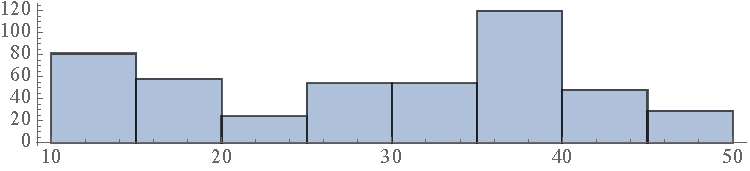
\includegraphics[width=.8\textwidth]{Figures/ACM/p-hist.pdf}
  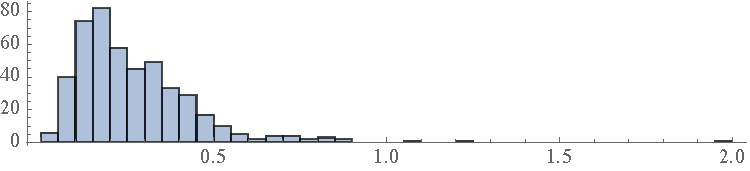
\includegraphics[width=.8\textwidth]{Figures/ACM/f-hist.pdf}
  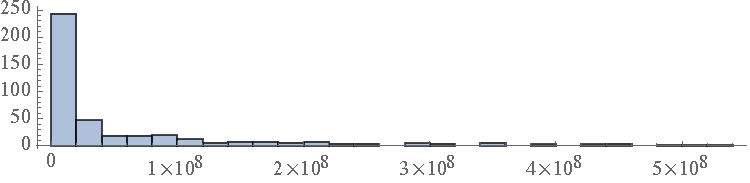
\includegraphics[width=.8\textwidth]{Figures/ACM/h-hist.pdf}
  \caption{Histograms of Parkinsons (total UPDRS), forest fire (area), and HPC I/O (mean throughput) response values respectively. Notice that both the forest fire and HPC I/O data sets are heavily skewed.
  \vspace{-.5cm}}
  \label{fig_response_hists}
\end{figure}

\subsection{High Performance Computing I/O ($n = 532, d = 4$)}
The first of three data sets is a four-dimensional data set produced by executing the IOzone benchmark from \cite{iozone} on a homogeneous cluster of computers. The system performance data was collected by executing IOzone 40 times for each of a select set of system configurations. A single IOzone execution reports the max I/O file-read throughput seen. The 40 executions for each system configuration are converted to their mean, which is capable of being modeled by each of the multivariate approximation techniques presented earlier in this chapter. The four dimensions being modeled to predict throughput mean are file size, record size, thread count, and CPU frequency.

\begin{figure*}[htb]
  \centering
  \begin{tikzpicture}
    \node (img)  {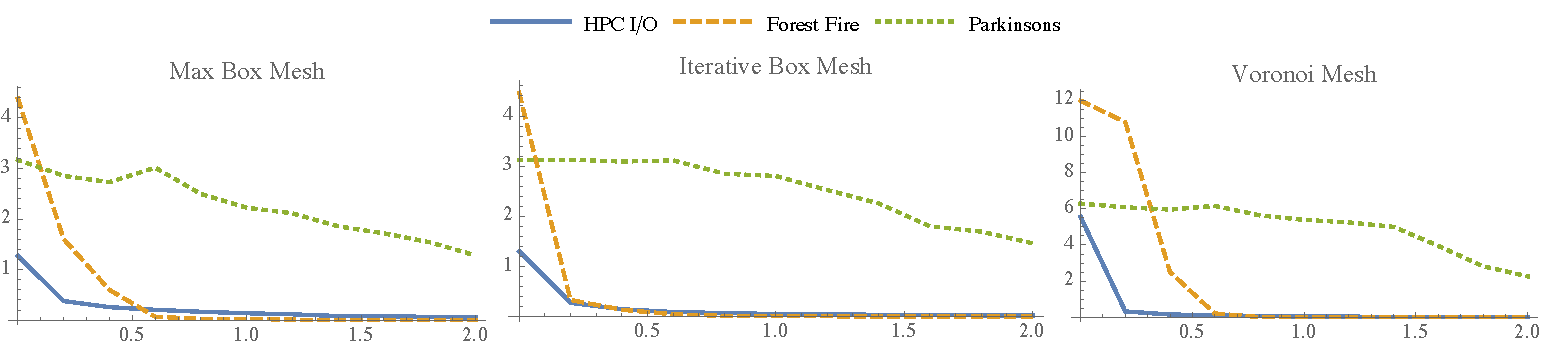
\includegraphics[width=0.95\textwidth,height=4cm]{Figures/ACM/eval-times.pdf}};
    \node[below=of img, node distance=0cm, yshift=1cm] {Relative Error Tolerance while Bootstrapping};
    \node[left=of img, node distance=0cm, rotate=90, anchor=center,yshift=-0.7cm] {Fit Time};
  \end{tikzpicture}
  \caption{Time required to generate model fits for each technique with varying relative error tolerance during bootstrapping.
    \vspace{-.3cm}}
  \label{fig_eval_times}
\end{figure*}

\subsection{Forest Fire ($n = 517, d = 12$)}
The forest fire data set \cite{cortez2007data} describes the area of Montesinho park burned on specific days and months of the year in terms of the environmental conditions. The twelve dimensions being used to model burn area are the $x$ and $y$ spatial coordinates of burns in the park, month and day of year, the FFMC, DMC, DC, and ISI indices (see source for details), the temperature in Celsius, relative humidity, wind speed, and outdoor rain. The original analysis of this data set demonstrated it to be difficult to model, likely due to the skew in response values.

\subsection{Parkinson's Telemonitoring ($n = 468, d = 16$)}
The final data set for evaluation \cite{tsanas2010accurate} is derived from a speech monitoring study with the intent to automatically estimate Parkinson's disease symptom development in Parkinson's patients. The function to be predicted is a time-consuming clinical evaluation measure referred to as the UPDRS score. The total UPDRS score given by a clinical evaluation is estimated through 16 real numbers generated from biomedical voice measures of in-home sound recordings.

\subsection{Performance Analysis}
\label{sec_performance_analysis}

The performance of the approximation techniques varies considerably across the three evaluation data sets. Relative errors for the most na\"{\i}ve approximators such as nearest neighbor can range from zero to $\displaystyle \big(\max_x f(x) - \min_x f(x)\big) / \min_x f(x)$ when modeling a positive function $f(x)$ from data. Each of the approximation techniques presented remain within these bounds and all errors are presented in signed relative form $(\hat f(x) - f(x)) / f(x)$. Before the models are constructed all data values (components $x^{(i)}_r$ of $x^{(i)} \in X$) are shifted and scaled to be in the unit cube $[0,1]^d$, while the response values are taken in their original form. All models are evaluated with $10$ random $80/20$ splits of the data.

\begin{table}
  \centering
  \begin{tabular}{c|c|c|c}
    \hline
    \textbf{Data Set} & \textbf{Technique} & \textbf{Tolerance} & \textbf{Average Error}\\
    \hline
    HPC I/O & MBM & 1.2 & 0.597\\
    Forest Fire & MBM & 1.8 & 3.517\\
    Parkinson's & MBM & 0.6 & 0.114\\
    \hline
    HPC I/O & IBM & 0.4 & 0.419\\
    Forest Fire & IBM & 1.8 & 3.615\\
    Parkinson's & IBM & 1.8 & 0.121\\
    \hline
    HPC I/O & VM & 0.2 & 0.382\\
    Forest Fire & VM & 1.0 & 4.783\\
    Parkinson's & VM & 2.0 & 1.824\\
    \hline
  \end{tabular}
  \caption{The optimal error tolerance bootstrapping parameters for each technique and each data set as well as the average absolute relative errors achieved by that tolerance. Notice that large relative error tolerances occasionally yield even lower evaluation errors, demonstrating the benefits of approximation over interpolation for noisy data sets.
  \vspace{-.5cm}}
  \label{tab_optimal_tolerance}
\end{table}

Each of the approximation techniques presented incorporates bootstrapping based on an allowable error tolerance $t$. An analysis of the effects of bootstrapping error tolerances on validation accuracy can be seen in Figure \ref{fig_all_performance}. The approximation meshes perform best on the forest fire and Parkinson's data sets when the error tolerance used for fitting is large (smoothing rather than interpolating), while near-interpolation generally produces the most accurate models for HPC I/O. Another performance result of note is that the $MBM$ and $IBM$ have very similar basis functions with largely different outputs.

\begin{figure*}
  \begin{tikzpicture}
    \node (img)  {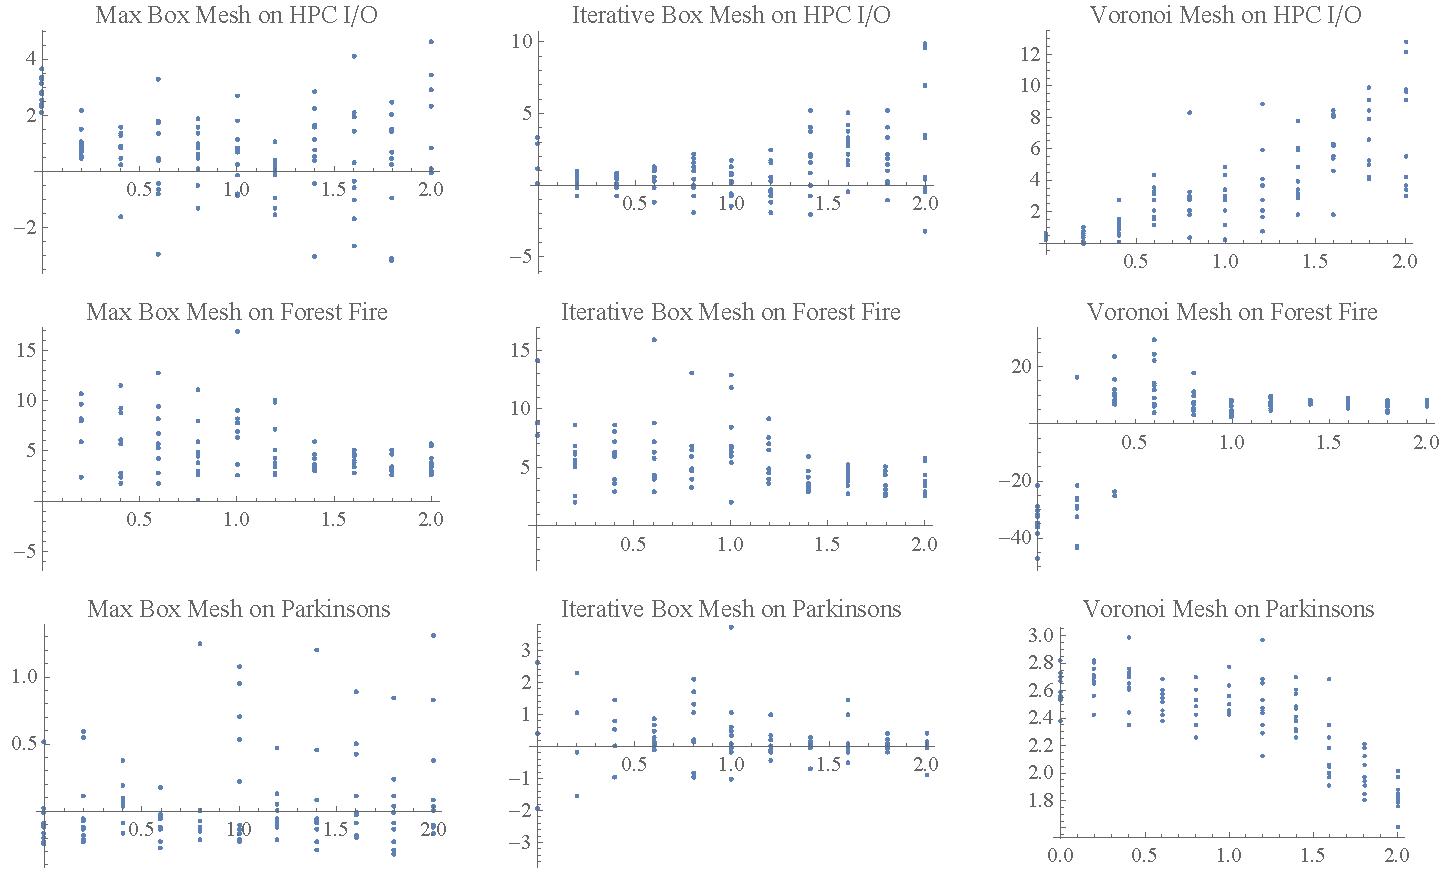
\includegraphics[width=0.95\textwidth,height=9.5cm]{Figures/ACM/all-performance.pdf}};
    \node[below=of img, node distance=0cm, yshift=1cm] {Relative Error Tolerance while Bootstrapping};
    \node[left=of img, node distance=0cm, rotate=90, anchor=center,yshift=-0.7cm] {Signed Relative Error};
  \end{tikzpicture}
  \caption{The performance of all three techniques with varied relative error tolerance for the bootstrapping parameter. The columns are for Max Box Mesh, Iterative Box Mesh, and Voronoi Mesh, respectively. The rows are for HPC I/O, Forest Fire, and Parkinson's respectively. Notice the techniques' behavior on the Parkinson's and Forest Fire data sets, performance increases with larger error tolerance.}
  \label{fig_all_performance}
\end{figure*}

\begin{figure*}
  \begin{tikzpicture}
    \node (img)  {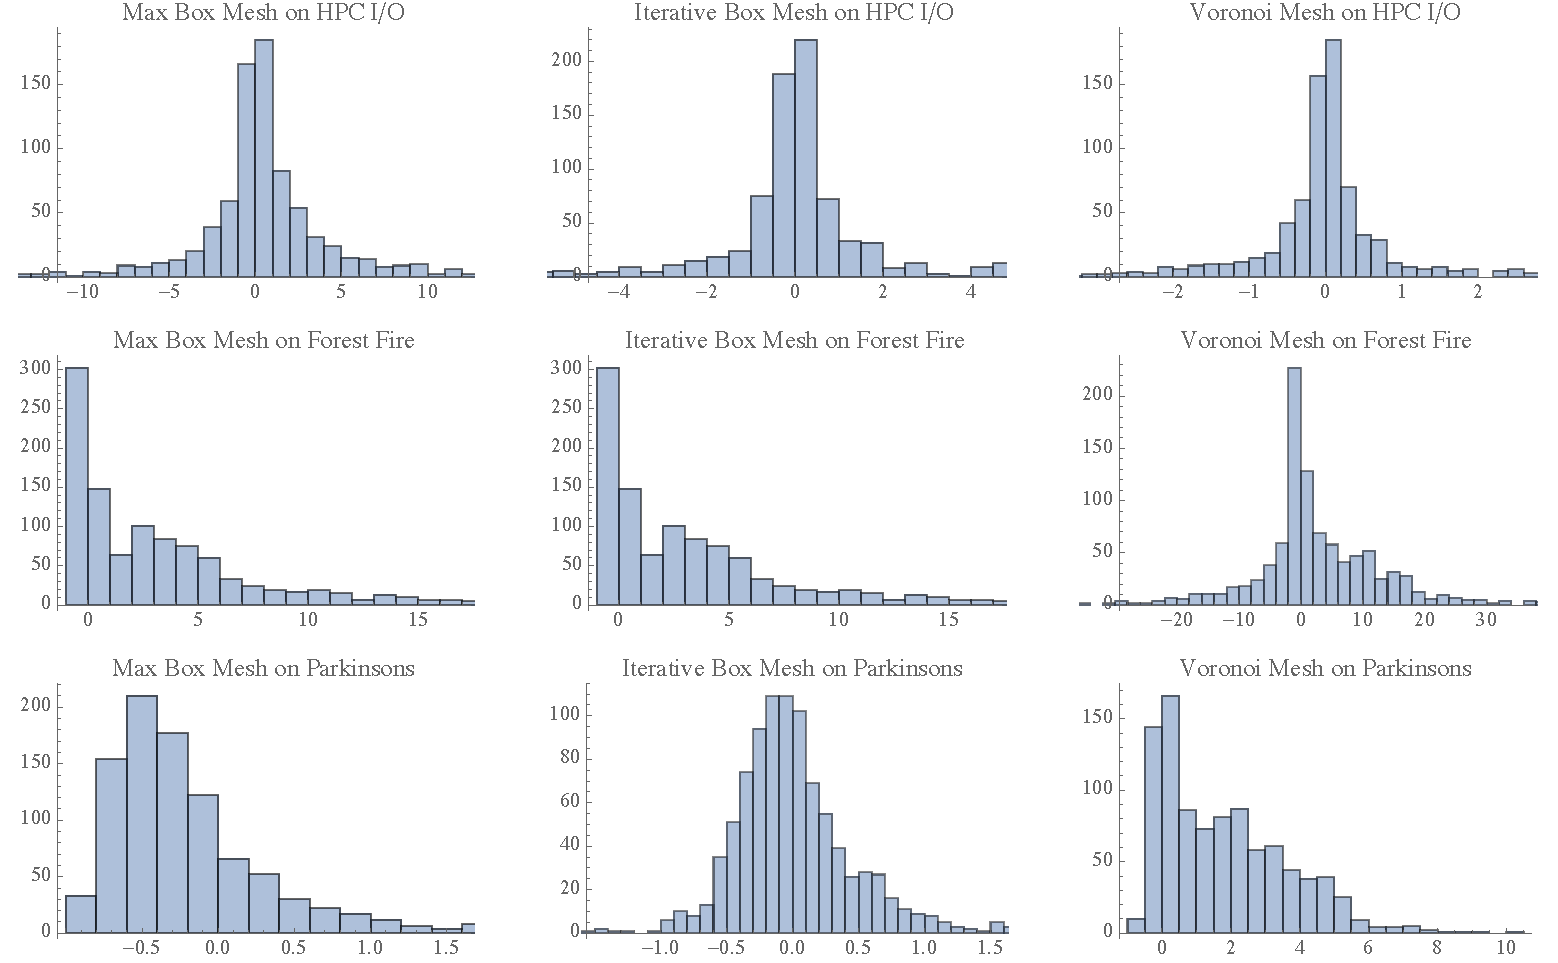
\includegraphics[width=0.95\textwidth,height=9.5cm]{Figures/ACM/perf-sample.pdf}};
    \node[below=of img, node distance=0cm, yshift=1cm] {Signed Relative Error in Prediction};
    \node[left=of img, node distance=0cm, rotate=90, anchor=center,yshift=-0.7cm] {Count};
  \end{tikzpicture}
  \caption{A sample of relative errors for all three techniques with optimal selections of error tolerance. The columns are for Max Box Mesh, Iterative Box Mesh, and Voronoi Mesh, respectively. The rows are for HPC I/O, Forest Fire, and Parkinson's respectively.
    \vspace{-.3cm}}
  \label{fig_perf_sample}
\end{figure*}

The selection of bootstrapping error tolerance also effects the computation time required to fit each of the models to data. Figure \ref{fig_eval_times} presents the time required to construct approximations for each model and each data set with varying $t$. The rapid reduction in computation time required for the forest fire and HPC I/O data sets suggests that large reductions in error can be achieved with relatively few basis functions. The Parkinson's data set however presents a more noisy response, with increasing number of basis functions reducing error much less quickly.

The distributions of errors experienced by each approximation technique when the optimal bootstrapping relative error tolerance is selected can be seen in Figure \ref{fig_perf_sample}. HPC I/O exhibits the most normal approximation errors, which suggests that the models are converging on the random noise of the response for the data set. The worst relative approximation errors are produced by the Voronoi mesh on the forest fire data set. The small magnitude true response values contribute to the larger relative errors. Regardless, the $VM$ errors are unacceptably large.

\section{Discussion of Mesh Approximations}

The bootstrapping procedure presented for each quasi-mesh approximation is very computationally expensive and does not provide much improvement over the interpolatory approach. Analysis suggests that the appropriate relative error tolerance needs to be discovered empirically for each application of a modeling technique. Further analytic studies could arrive at methods for determining optimal error tolerances at runtime, however increases in runtime complexity may not be afforded in many applications. 

The box-shaped basis functions and the construction algorithms used for the $MBM$ and $IBM$ could become a source of error when $d$ (the dimension of the data $X$) is comparable to $n$ (the number of known points). The blending regions in which multiple basis functions overlap are always axis aligned and in applications such as image analysis, any single dimension may be unsuitable for approximating the true underlying function. The Voronoi mesh attempts to address this problem by utilizing boundaries between points in multiple dimensions simultaneously. However, it is empirically unclear whether the true benefits of the $VM$ are seen in applications where $d \ll n$.

Each of the case studies presented have fewer than $1000$ points. The complexity of the presented approximation techniques are suitable for large dimension, but the increased complexity associated with brute-force bootstrapping prohibits their use on larger data sets. The Voronoi mesh in particular has a large complexity with respect to $n$ which could be significantly improved by dropping bootstrapping, as is done in Chapter \ref{ch:strong}. While each technique requires less than ten seconds on average to produce a fit in the presented case studies, the fit time required quickly grows into minutes around $1000$ points. These results demonstrate the limits of expensive bootstrapping. However, the viability of each mesh encourages the further applications explored in later chapters.

\section{Implications of Quasi-Mesh Results}

The Max Box Mesh, Iterative Box Mesh, and Voronoi Mesh each provide novel strategies for effectively approximating multivariate phenomonon. The underlying constructions are theoretically straightforward. The computational complexities of each make them particularly suitable for applications in many dimensions, while the bootstrapping error tolerance parameter allows a balance between smoothing and interpolation to be explored empirically with each application. However, the expense of bootstrapping prohibits its use on larger data sets.

